\section{Empirical application and results}\label{sec:results}
We ask whether GPS-signed synthetic comparisons yield a policy that retains country ordering on a separate survey, and whether that ordering agrees with WVS respondents.

The diagnostic panel is Argentina, Brazil, China, Germany, Egypt, Great Britain, Greece, Indonesia, India, Japan, Mexico, Nigeria, the Netherlands, Russia, Turkey, and the United States. These sixteen countries are the complete census of adapters fitted in two production waves. The first wave covers China, Japan, Great Britain, the United States, Mexico, Argentina, Germany, and Russia. The second covers India, Indonesia, Nigeria, Egypt, Turkey, the Netherlands, Brazil, and Greece. We assembled those waves to include both global sign polarities, the three twin pairs that share a labeling problem, mixed profiles, and geographic spread. That is, the panel is a census of fitted production adapters. It is not a probability sample of the forty-two-country GPS--WVS intersection. A later study that treats country selection as a sampling problem should train every country in that intersection or a predeclared random subset of it.

The primary comparison holds countries, item sets, recodes, and aggregation rules fixed across arms. It contains twenty-three single-choice items, including nine trust items. Egypt has no valid Q69--Q71 observations and Great Britain has no valid Q174 observations, so these items are removed everywhere. Q12--Q14 are multiple-response items and are excluded from the categorical softmax evaluation. Table~\ref{tab:map} lists the resulting map. Its proposed composites should not be read as validated measures of all six GPS traits. The original mapping preceded model scoring, whereas the strict common-support analysis and its sensitivity checks are retrospective.

\begin{table}[htbp]\centering\small
\caption{Candidate indicators on the strict common-support panel. Each row defines a candidate item set; latent-scale validity remains to be assessed. Patience items are interpreted separately.}\label{tab:map}
\begin{tabularx}{\linewidth}{@{}>{\raggedright\arraybackslash}p{30mm}>{\raggedright\arraybackslash}p{35mm}>{\raggedright\arraybackslash}X@{}}\toprule
Anchor & WVS items & Interpretation to be assessed\\\midrule
Trust & Q57--Q64, Q73 & Generalized, interpersonal, and institutional trust/confidence\\
Patience & Q43; Q50 & Less importance placed on work; financial satisfaction\\
Risk taking & Q106, Q107, Q109, Q178 & Economic values and fare avoidance\\
Positive reciprocity & Q81 & Confidence in charitable organizations\\
Negative reciprocity & Q176, Q177, Q179, Q195 & Moral clarity and justifiability judgments\\
Altruism & Q99, Q101, Q103 & Membership in environmental, charitable, and self-help groups\\\bottomrule
\end{tabularx}\end{table}

GPS supplies prior economic-preference benchmarks. Equivalence between each listed WVS item and its proposed GPS measure remains to be assessed. Q57 is the generalized-trust item related to the GPS validation comparison \cite{falk2018}; its human--GPS association in our sixteen-country panel is only $0.15$. The wider trust composite pools substantively different items. The other mappings are exploratory bridges, especially where Wave~7 has no direct counterpart to the preference measure.

\subsection{Recovery of the synthetic labels}
Each country adapter uses 526 training comparisons from a shared 658-pair bank, with 132 held-out comparisons. The fitting configuration uses $\beta=0.1$, LoRA rank 16 and scaling parameter 32, and one epoch. The countries instantiate thirteen distinct six-sign profiles (Table~\ref{tab:signprofiles}): Mexico shares its signs with Russia, India with Greece, and Indonesia with Egypt. Thus there are fewer distinct labeling problems than country labels. Appendix~\ref{app:training} records configuration and provenance limits.
\begin{table}[htbp]\centering\small
\caption{Thirteen distinct GPS sign profiles among the sixteen adapter countries. Coordinates are ordered trust, risk taking, patience, altruism, positive reciprocity, and negative reciprocity, matching Appendix~\ref{app:protocol}. The United States is non-negative on every coordinate; Mexico and Russia are negative on every coordinate. Identical sign vectors induce identical labels on the shared bank.}\label{tab:signprofiles}
\begin{tabular}{lcccccc}\toprule
Members & trust & risk & patience & altruism & pos.\ recip. & neg.\ recip. \\\midrule
EGY, IDN & $+$ & $-$ & $-$ & $+$ & $+$ & $+$ \\
GRC, IND & $-$ & $-$ & $-$ & $-$ & $-$ & $+$ \\
MEX, RUS & $-$ & $-$ & $-$ & $-$ & $-$ & $-$ \\
ARG & $-$ & $+$ & $-$ & $+$ & $+$ & $-$ \\
BRA & $-$ & $-$ & $-$ & $+$ & $+$ & $-$ \\
CHN & $+$ & $-$ & $+$ & $+$ & $+$ & $+$ \\
DEU & $-$ & $-$ & $+$ & $-$ & $-$ & $-$ \\
GBR & $+$ & $+$ & $+$ & $+$ & $-$ & $+$ \\
JPN & $-$ & $-$ & $+$ & $-$ & $-$ & $+$ \\
NGA & $-$ & $+$ & $-$ & $-$ & $-$ & $+$ \\
NLD & $+$ & $+$ & $+$ & $-$ & $-$ & $+$ \\
TUR & $+$ & $+$ & $-$ & $-$ & $-$ & $+$ \\
USA & $+$ & $+$ & $+$ & $+$ & $+$ & $+$ \\
\bottomrule
\end{tabular}\end{table}


Pair-pooled across 2,112 held-out country--pair cells, relative-reward recovery is $0.942$ and raw adapter choice accuracy is $0.819$. The former records a positive improvement in the chosen--rejected margin over the reference; the latter records a positive adapted-model margin itself. Country-level relative-reward recovery ranges from $0.886$ to $0.992$. These results support recovery of imposed synthetic contrasts. They do not measure prediction of independently observed choices. Fifteen countries share the seed-42 holdout; Russia's different 132-pair holdout shares 26 prompts with that set. This limits interpretation of pooled precision and country comparisons.

\subsection{Cross-survey associations}
Figure~\ref{fig:associations} compares human--GPS, adapter--GPS, adapter--human, and persona--human associations on the matched panel. Table~\ref{tab:persona} supplies the otherwise missing persona--GPS comparator. Country-bootstrap intervals use 2,000 common resamples and describe sensitivity conditional on the fitted policies, GPS anchors, WVS point estimates, and selected items. They do not include respondent sampling, anchor measurement error, or training randomness, and are not multiplicity-adjusted.

\begin{figure}[htbp]\centering
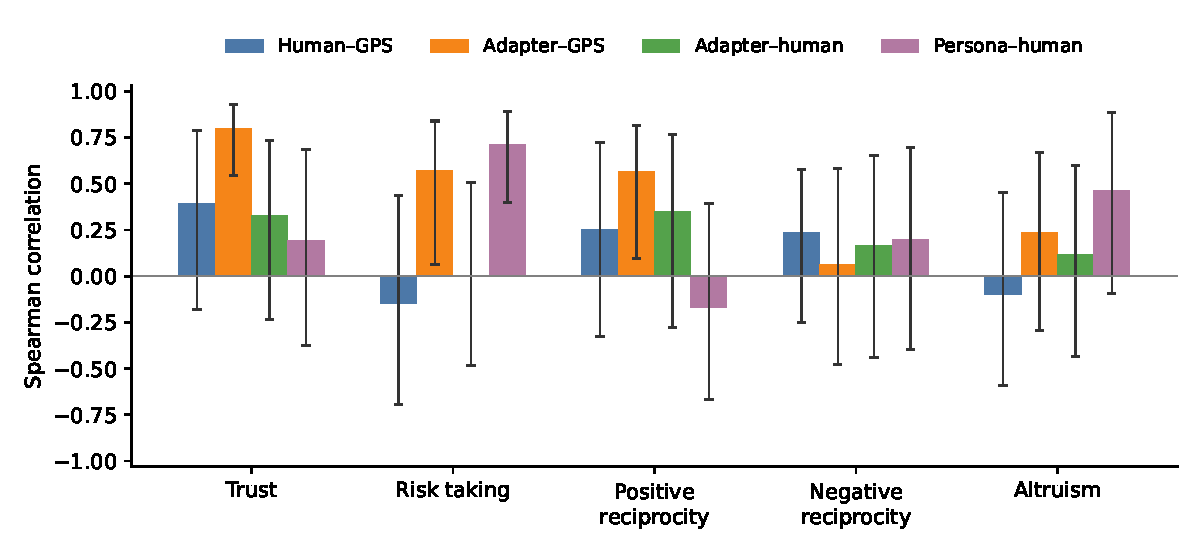
\includegraphics[width=\linewidth]{figures/associations.pdf}
\caption{Strict sixteen-country panel: country-rank associations with 95\% country-bootstrap intervals. Intervals exclude training-seed variation, respondent resampling, and GPS measurement error. The four series answer different questions; agreement with the anchor is distinct from agreement with human responses. Patience is omitted here because Q43 and Q50 have opposing human associations and is reported itemwise in Table~\ref{tab:patience}.}\label{fig:associations}
\end{figure}

For trust, adapter--GPS association is $0.80$ $[0.55,0.93]$, compared with $-0.07$ for the persona arm. The paired adapter-minus-persona difference is $0.87$ $[0.22,1.36]$. Human--GPS association on the sixteen-country rectangle is $0.39$ $[-0.18,0.79]$, and adapter--human association is $0.33$ $[-0.23,0.74]$. The clearer finding is retention of anchor ordering on new trust text. The sixteen-country intervals leave human agreement unresolved, and they also leave the map's own criterion association unresolved. On the same nine-item recodes, the forty-two-country GPS--WVS intersection yields human--GPS association $0.35$ $[0.09,0.56]$ (Table~\ref{tab:human42}). That larger human panel is a criterion check on the map. Adapters are not retrained, and the adapter--human interval is unchanged. Similarity between a correlation and a product of two other correlations would not identify a mechanism, so we draw no such inference.

\begin{table}[htbp]\centering\small
\caption{Country-named persona--GPS association on the strict panel, with 95\% country-bootstrap intervals. This supplies the anchor comparator for Figure~\ref{fig:associations}.}\label{tab:persona}
\begin{tabular}{lcc}\toprule Anchor & $\rho$ & Interval\\\midrule
Trust & -0.07 & [-0.55, 0.45] \\
Risk taking & -0.11 & [-0.72, 0.51] \\
Positive reciprocity & 0.02 & [-0.47, 0.48] \\
Negative reciprocity & 0.34 & [-0.17, 0.82] \\
Altruism & -0.23 & [-0.64, 0.26] \\
\bottomrule
\end{tabular}\end{table}


Risk taking shows why the targets must remain distinct. Adapter--GPS association is $0.57$, human--GPS is $-0.15$, and adapter--human is exactly zero in this sample, with interval $[-0.48,0.51]$. The zero records zero sample rank association; it establishes neither independence nor different latent constructs. Persona--human association is $0.71$ while persona--GPS is $-0.11$. Mapping choices, anchor measurement, ecological differences, bank semantics, and fitting or scoring limitations can all contribute to this divergence. Positive reciprocity has only Q81 on the strict panel. Negative reciprocity and altruism likewise provide no resolved adapter--human result.

\begin{table}[htbp]\centering\small
\caption{Patience candidate indicators, separately scored on sixteen countries. Entries are Spearman correlations; brackets give 95\% country-bootstrap intervals.}\label{tab:patience}
\begin{tabular}{lcc}\toprule Pairing & Q43 & Q50\\\midrule
Human--GPS & -0.56 [-0.86, -0.04] & 0.62 [0.11, 0.91] \\
Adapter--GPS & 0.01 [-0.47, 0.44] & 0.44 [-0.12, 0.79] \\
Adapter--human & 0.29 [-0.19, 0.73] & 0.25 [-0.32, 0.70] \\
Persona--GPS & -0.62 [-0.90, -0.10] & 0.62 [0.16, 0.87] \\
Persona--human & 0.59 [0.11, 0.82] & 0.70 [0.23, 0.91] \\
\bottomrule
\end{tabular}\end{table}

The two patience items have opposite human--GPS signs (Table~\ref{tab:patience}). Q43 concerns reduced importance of work, whereas Q50 concerns financial satisfaction. We retain their original coding and report them separately rather than selecting a polarity after observing the correlations. Their two-item mean is an available computational summary, but it is not treated as a validated patience measure. The main interpretation therefore does not use its aggregate correlation.

Retrospective influence checks leave trust adapter--GPS association between $0.779$ and $0.850$ when one country is omitted, and between $0.659$ and $0.847$ when one trust item is omitted. Resampling thirteen whole sign profiles gives $0.80$ $[0.45,0.92]$; equal weighting of profile means gives $0.85$ $[0.53,0.98]$. These are within-panel sensitivity checks. They do not demonstrate transport to new countries or independently generated scenario banks. Permuting the sixteen GPS trust scores across the frozen adapter composites, without refitting, yields a null median near zero and one-sided $p=0.002$ (seed 20260820; 1,000 draws). That assignment check is not a sign-retrain test. Appendix~\ref{app:measurement} reports the paired Egypt and Q69--Q71 surfaces.

\subsection{Distributional fit and prompt sensitivity}
Table~\ref{tab:twobytwo} compares configurations on the same twenty-three-item surface. Adding a persona prompt to an adapter yields trust--GPS association $0.67$, below the unconditioned adapter's $0.80$. The persona baseline has lower TVD than either adapter configuration. Directional anchor retention and closeness to human response distributions therefore need not favor the same configuration.

\begin{table}[htbp]\centering\small
\caption{Configuration sensitivity on the strict panel. TVD averages 368 country--item cells. The adapter--persona row uses the space-prefixed rescore. The base TVD uses banked runs; no base country-ordering estimate is interpreted because run variation is confounded with bank. Rank associations on this table use the same country bootstrap as Figure~\ref{fig:associations}, which excludes training-seed variation and GPS measurement error.}\label{tab:twobytwo}
\begin{tabular}{lcc}\toprule
Configuration & Trust--GPS $\rho$ & Mean TVD\\\midrule
Base, unconditioned & --- & 0.462\\
Base, persona & $-0.07$ & 0.369\\
Adapter, unconditioned & 0.80 & 0.480\\
Adapter, persona & 0.67 & 0.401\\\bottomrule
\end{tabular}\end{table}

The pattern is dimension-dependent. With a country prompt, risk adapter--GPS association changes from $0.57$ to $-0.26$ and adapter--human changes from zero to $0.62$. These changes describe configuration sensitivity. They do not separate latent priors from anchor effects or establish a general division between weights determining direction and prompts determining shape. The historical base runs also vary numerically despite identical saved prompts. A single fixed base distribution would have undefined country-rank association on the common item set. Full checkpoint, tokenizer, and realized-prompt equivalence across runs remains a release gate.

The earlier rewrite also reported a broader thirty-item shape diagnostic. We do not mix its TVD levels with the strict-panel estimates, and omit its exhibit pending reconciliation of item eligibility and historical aggregation. In particular, an ordering result alone cannot establish population dispersion. The evidence supports a fitted synthetic policy with trait-dependent external anchor association; reliable prediction of human country ranks and practical pre-pilot benefits remain unestablished.
